\documentclass{beamer}
\usepackage{amsmath}
\usepackage{amssymb}
\usepackage{graphicx}
\usepackage{xcolor}
\usepackage{listings}
\usepackage{algorithm}
\usepackage{algpseudocode}
\usepackage{tikz}
\usepackage{empheq}
\usepackage{xcolor}  % Load xcolor first
\usepackage{listings}

\lstdefinelanguage{JavaScript}{
    keywords={break, case, catch, continue, debugger, default, delete, do, else, finally,
              for, function, if, in, instanceof, new, return, switch, this, throw, try,
              typeof, var, void, while, with, const, let},
    sensitive=true,
    comment=[l]{//}, 
    morecomment=[s]{/*}{*/},
    morestring=[b]",
    morestring=[b]'
}

\lstset{
    language=JavaScript,
    basicstyle=\small\ttfamily,
    numbers=left,
    numberstyle=\tiny,
    stepnumber=1,
    numbersep=5pt,
    keywordstyle=\color{blue},
    commentstyle=\color{green!50!black},
    stringstyle=\color{red},
}



% Theme configuration
\usetheme{Madrid}
\usecolortheme{default}
\setbeamertemplate{navigation symbols}{}
\setbeamertemplate{footline}[frame number]

 
\begin{document}

\begin{frame}{ Discretize the Domain}
    \begin{itemize}
        \onslide<2->{
            \item $u_{i,j}^k$ represents the concentration $u(x_i, y_j, t_k)$
        }
        \onslide<3->{
            \item Space discretization: $(x_i, y_j)$ where $x_i = i\Delta x$  and $y_j = j\Delta y$ 

        }
        \onslide<4->{   
            \item Time discretization: $t_k = k\Delta t$ for $k = 0,1,...$

        }
    \end{itemize}

       \begin{figure}
        \onslide<1->{
            \centering
            \begin{minipage}{0.29\textwidth}
                \centering
                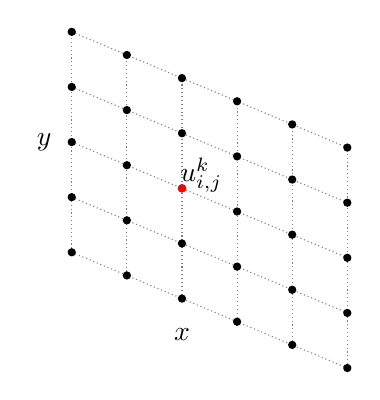
\begin{tikzpicture}[scale=0.7]
                    \foreach \y in {0,...,4}
                        \draw[gray, densely dotted] (0,\y) -- (5,\y-5*0.42);
                    
                    \foreach \x in {0,...,5}
                        \draw[gray, densely dotted] (\x,0-\x*0.42) -- (\x,4-\x*0.42);
                    
                    \foreach \x in {0,...,5}
                        \foreach \y in {0,...,4} {
                            \fill (\x,\y-\x*0.42) circle (0.0753);
                            \ifnum \x=2 \ifnum \y=2
                                \fill[red] (\x,\y-\x*0.42) circle (0.0753);
                            \fi \fi
                        }
                         
                          
                    \node at (2.0, -1.5) {$x$};
                    \node at (-0.5, 2) {$y$};
                    \node at (2.35, 1.4) {$u_{i,j}^k$};
                \end{tikzpicture}
            \end{minipage}
        }
        \onslide<5->{
            \hspace{0.4cm}
            \begin{minipage}{0.29\textwidth}
                \centering
                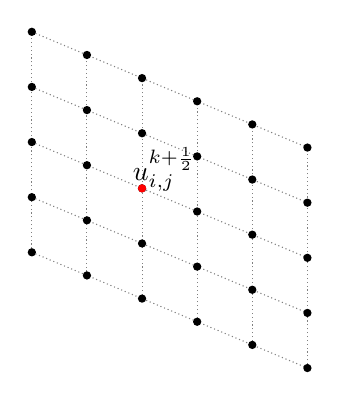
\begin{tikzpicture}[scale=0.7]
                    \foreach \y in {0,...,4}
                        \draw[gray, densely dotted] (0,\y) -- (5,\y-5*0.42);
                    
                    \foreach \x in {0,...,5}
                        \draw[gray, densely dotted] (\x,0-\x*0.42) -- (\x,4-\x*0.42);
                    
                        \foreach \x in {0,...,5}
                        \foreach \y in {0,...,4} {
                            \fill (\x,\y-\x*0.42) circle (0.0753);
                            \ifnum \x=2 \ifnum \y=2
                                \fill[red] (\x,\y-\x*0.42) circle (0.0753);
                            \fi \fi
                        }
                    
                    \node at (2.4, 1.5) {$u_{i,j}^{k+\frac{1}{2}}$};
                \end{tikzpicture}
            \end{minipage}
        }
        \onslide<4->{
            \begin{minipage}{0.29\textwidth}
                \centering
                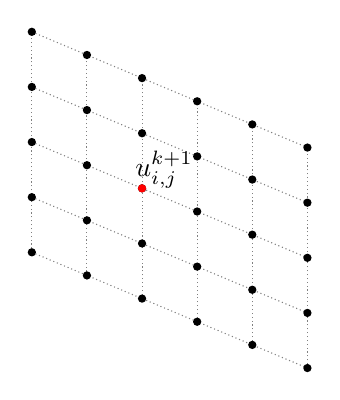
\begin{tikzpicture}[scale=0.7]
                    \foreach \y in {0,...,4}
                        \draw[gray, densely dotted] (0,\y) -- (5,\y-5*0.42);
                    
                    \foreach \x in {0,...,5}
                        \draw[gray, densely dotted] (\x,0-\x*0.42) -- (\x,4-\x*0.42);
                    
                        \foreach \x in {0,...,5}
                        \foreach \y in {0,...,4} {
                            \fill (\x,\y-\x*0.42) circle (0.0753);
                            \ifnum \x=2 \ifnum \y=2
                                \fill[red] (\x,\y-\x*0.42) circle (0.0753);
                            \fi \fi
                        } 
                            \node at (2.4, 1.5) {$u_{i,j}^{k+1}$};
                        \end{tikzpicture}
            \end{minipage}
            }
        \end{figure} 
        
        \begin{center}
        \begin{tikzpicture}[>=stealth]
            % Time arrow with specific steps
            \onslide<4->{
            \draw[->] (0,0) -- (11,0) node[label=above:Time] {};}
            
            % Time points and labels
            \onslide<4->{
            \fill (2,0) circle (0.1) node[below] {$k$};}
            \onslide<5->{
            \fill (5.5,0) circle (0.1) node[below] {$k+\frac{1}{2}$};}
            \onslide<4->{
            \fill (9,0) circle (0.1) node[below] {$k+1$};}
          
        \end{tikzpicture}
        \end{center}
\end{frame}
\begin{frame}{Simulationg point-like sinks and sources}
    \vspace{-0.5cm}
    \onslide<1->{
        \begin{align*}
            \frac{\partial u}{\partial t} &= 
            D\Biggl( \frac{\partial^2 u}{\partial x^2} + \frac{\partial^2 u}{\partial y^2} \Biggr) 
            + \sum_{b=1}^{N}  K_{out}(c_b)\delta(r_b - r)
            - K_{in}(u) \sum_{b=1}^{N} \delta(r_b - r)
        \end{align*}
    }
    \onslide<2->{
        We can discretize the first half-step ($x$ implicit, $y$ explicit) using the following scheme:

        \vspace{-0.5cm}
             {\small % Optionally reduce font size
        \begin{equation*}
            \frac{u_{i,j}^{k+\frac{1}{2}} - u_{i,j}^{k}}{\Delta t/2}
            = D\Biggl(
            \frac{u_{i+1,j}^{k+\frac{1}{2}} - 2u_{i,j}^{k+\frac{1}{2}} + u_{i-1,j}^{k+\frac{1}{2}}}{\Delta x^2} + \frac{u_{i,j+1}^{k} - 2u_{i,j}^{k} + u_{i,j-1}^{k}}{\Delta y^2}
            \Biggr)
            + S^k
        \end{equation*}
        }
    }
     \onslide<3->{
        And the second half-step ($x$ explicit, $y$ implicit) using the following scheme:
        \vspace{-0.1cm}
        {\small % Optionally reduce font size
        \begin{equation*}
            \frac{u_{i,j}^{k+1} - u_{i,j}^{k+\frac{1}{2}}}{\Delta t/2}
            = D\Biggl(
            \frac{u_{i+1,j}^{k+\frac{1}{2}} - 2u_{i,j}^{k+\frac{1}{2}} + u_{i-1,j}^{k+\frac{1}{2}}}{\Delta x^2} + \frac{u_{i,j+1}^{k+1} - 2u_{i,j}^{k+1} + u_{i,j-1}^{k+1}}{\Delta y^2}
            \Biggr)
            + S^{k+\frac{1}{2}}
        \end{equation*}
        }
     }
     \onslide<4->{
        
       Where $S$ is the sources and sinks term:
        \begin{align*}
            S^k =  \sum_{b=1}^{N}K_{out}(c_b) \delta_{\varepsilon}(r_b - r_{i,j})-  K_{in} (u^k_{i,j}) \sum_{b=1}^{N} \delta_{\varepsilon}(r_b - r_{i,j})
        \end{align*}
        }
    
\end{frame}

\begin{frame}
    Let's start with the first half-step:

       \onslide<1->{

        \vspace{-0.5cm}
             {\small % Optionally reduce font size
        \begin{equation*}
            \frac{u_{i,j}^{k+\frac{1}{2}} - u_{i,j}^{k}}{\Delta t/2}
            = D\Biggl(
            \frac{u_{i+1,j}^{k+\frac{1}{2}} - 2u_{i,j}^{k+\frac{1}{2}} + u_{i-1,j}^{k+\frac{1}{2}}}{\Delta x^2} + \frac{u_{i,j+1}^{k} - 2u_{i,j}^{k} + u_{i,j-1}^{k}}{\Delta y^2}
            \Biggr)
            +  S^k
        \end{equation*}
        }
    }
    \onslide<2->{
    \vspace{0.0cm}
To simplify, we notice that $\Delta x = \Delta y$, and we can define $\alpha = \frac{D \Delta t}{2 \Delta x^2}$ to get:
\vspace{-0.5cm}
        \begin{equation*}
           u_{i,j}^{k+\frac{1}{2}} - u_{i,j}^{k}
            = \alpha\Biggl(
            u_{i+1,j}^{k+\frac{1}{2}} - 2u_{i,j}^{k+\frac{1}{2}} + u_{i-1,j}^{k+\frac{1}{2}}+ u_{i,j+1}^{k} - 2u_{i,j}^{k} + u_{i,j-1}^{k}
            \Biggr)
            + \frac{\Delta t}{2}S^k
        \end{equation*} 
    }
    \onslide<3->{
Now we can rearrange the equation to isolate the unknown terms $u_{i,j}^{k+\frac{1}{2}}$ on the left-hand side:
    \begin{align*}
        \resizebox{\textwidth}{!}{%
$\boxed{\small 
\colorbox{red!20}{$ -\alpha u_{i-1,j}^{k+\frac{1}{2}} + (1 + 2\alpha)u_{i,j}^{k+\frac{1}{2}} - 
\alpha u_{i+1,j}^{k+\frac{1}{2}} $}= 
\colorbox{blue!20}{$\alpha u_{i,j-1}^k + (1 - 2\alpha)u_{i,j}^k + \alpha u_{i,j+1}^k
+ 
\frac{\Delta t}{2} S^k$}}$}
\end{align*}
    We know all the terms in right-hand side of the equation (blue), but we need to compute the left-hand side (red). 

}
\end{frame}

\begin{frame}{First half-step ($x$ implicit, $y$ explicit)}
    \vspace{-1cm}
      \begin{align*}
        \resizebox{\textwidth}{!}{%
$\boxed{\small 
\colorbox{red!20}{$ -\alpha u_{i-1,j}^{k+\frac{1}{2}} + (1 + 2\alpha)u_{i,j}^{k+\frac{1}{2}} - 
\alpha u_{i+1,j}^{k+\frac{1}{2}} $}= 
\colorbox{blue!20}{$\alpha u_{i,j-1}^k + (1 - 2\alpha)u_{i,j}^k + \alpha u_{i,j+1}^k
+ 
\frac{\Delta t}{2} S^k$}}$}
\end{align*}
    \onslide<2->{
    \vspace{-0.5cm}
    Let's look around $i = 3$ and $j = 2$:
    \vspace{0.5cm}
    }
    \begin{figure}
            \centering
            \begin{minipage}{0.49\textwidth}
                \centering
                \onslide<3->{
                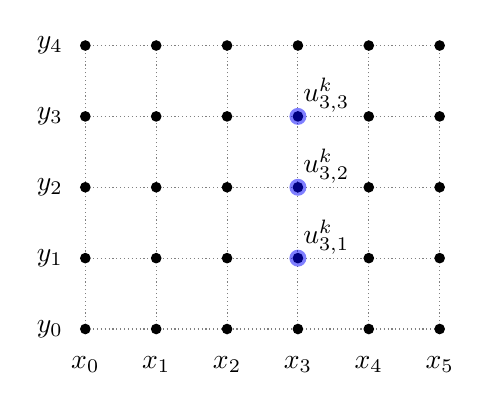
\begin{tikzpicture}[scale=0.9]
                   \foreach \y in {0,...,4} {
                        \draw[gray, densely dotted] (0,\y) -- (5,\y);
                        \node at (-0.5, \y) {$y_{\y}$};
                    }
                                        
                    \foreach \x in {0,...,5} {
                        \draw[gray, densely dotted] (\x,0) -- (\x,4);
                        \node at (\x, -0.5) {$x_{\x}$};
                    }
                    \foreach \x in {0,...,5}
                        \foreach \y in {0,...,4} {
                            \fill (\x,\y) circle (0.0753);
                           
                            \ifnum \x=3 \ifnum \y=1
                                \fill[blue,fill opacity=0.5 ] (\x,\y) circle (0.12);
                            \fi \fi
                            \ifnum \x=3 \ifnum \y=2
                                \fill[blue,fill opacity=0.5 ] (\x,\y) circle (0.12);
                            \fi \fi
                            \ifnum \x=3 \ifnum \y=3
                                \fill[blue,fill opacity=0.5 ] (\x,\y) circle (0.12);
                            \fi \fi
                        }
                    \node at (3.4, 2.3) {$u_{3,2}^k$};
                    \node at (3.4, 1.3) {$u_{3,1}^k$};
                    \node at (3.4, 3.3) {$u_{3,3}^k$};
                \end{tikzpicture}
                }
            \end{minipage}%
            \begin{minipage}{0.49\textwidth}
                \centering
                \onslide<4->{
                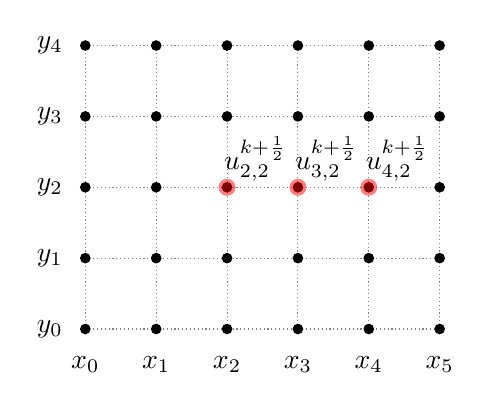
\begin{tikzpicture}[scale=0.9]
                    \foreach \y in {0,...,4} {
                        \draw[gray, densely dotted] (0,\y) -- (5,\y);
                        \node at (-0.5, \y) {$y_{\y}$};
                    }
                                        
                    \foreach \x in {0,...,5} {
                        \draw[gray, densely dotted] (\x,0) -- (\x,4);
                        \node at (\x, -0.5) {$x_{\x}$};
                    }
                    \foreach \x in {0,...,5}
                        \foreach \y in {0,...,4} {
                            \fill (\x,\y) circle (0.0753);
                          
                            \ifnum \x=3 \ifnum \y=2
                                \fill[red,fill opacity=0.5 ] (\x,\y) circle (0.12);
                            \fi \fi
                            \ifnum \x=2 \ifnum \y=2
                            \fill[red,fill opacity=0.5 ] (\x,\y) circle (0.12);
                        \fi \fi
                        \ifnum \x=4 \ifnum \y=2
                        \fill[red,fill opacity=0.5 ] (\x,\y) circle (0.12);
                    \fi \fi
                        }
                    \node at (3.4, 2.4) {$u_{3,2}^{k+\frac{1}{2}}$};
                    \node at (2.4, 2.4) {$u_{2,2}^{k+\frac{1}{2}}$};
                    \node at (4.4, 2.4) {$u_{4,2}^{k+\frac{1}{2}}$};
                \end{tikzpicture}
                }
            \end{minipage}
        \end{figure}
\end{frame}


\begin{frame}
    \vspace{-0.8cm}   
    Let's fix $j = 0$ and write the equations for $0 \leq i \leq 5$.
    
    \begin{columns}
        \begin{column}{0.3\textwidth}
            % Place both figures in a row here
            \begin{minipage}{0.2\textwidth}
                $k$
                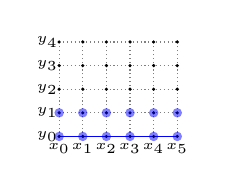
\begin{tikzpicture}[scale=0.3]
                    \foreach \y in {0,...,4} {
                         \draw[gray, densely dotted] (0,\y) -- (5,\y);
                         \node at (-0.5, \y) {\tiny$y_{\y}$};
                         \ifnum \y = 1
                            \draw[blue, thin] (0,0) -- (5,0);
                         \fi
                     }
                                         
                     \foreach \x in {0,...,5} {
                         \draw[gray, densely dotted] (\x,0) -- (\x,4);
                         \node at (\x, -0.5) {\tiny$x_{\x}$};
                     }
                     \foreach \x in {0,...,5}
                         \foreach \y in {0,...,4} {
                             \fill (\x,\y) circle (0.0753);
                             \onslide<3->{  
                             \ifnum \x=0 \ifnum \y=-1
                                 \fill[blue, fill opacity=0.5] (\x,\y) circle (0.2);
                             \fi \fi
                             \ifnum \x=0\ifnum \y=0
                                 \fill[blue, fill opacity=0.5] (\x,\y) circle (0.2);
                             \fi \fi
                             \ifnum \x=0 \ifnum \y=1
                                 \fill[blue, fill opacity=0.5] (\x,\y) circle (0.2);
                             \fi \fi
                             }
                            \onslide<4->{
                                \ifnum \x=1 \ifnum \y=-1
                                    \fill[blue, fill opacity=0.5] (\x,\y) circle (0.2);
                                \fi \fi
                                \ifnum \x=1\ifnum \y=0
                                    \fill[blue, fill opacity=0.5] (\x,\y) circle (0.2);
                                \fi \fi
                                \ifnum \x=1 \ifnum \y=1
                                    \fill[blue, fill opacity=0.5] (\x,\y) circle (0.2);
                                \fi \fi
                                }
                            \onslide<5->{
                                \ifnum \x=2 \ifnum \y=-1
                                    \fill[blue, fill opacity=0.5] (\x,\y) circle (0.2);
                                \fi \fi
                                \ifnum \x=2\ifnum \y=0
                                    \fill[blue, fill opacity=0.5] (\x,\y) circle (0.2);
                                \fi \fi
                                \ifnum \x=2 \ifnum \y=1
                                    \fill[blue, fill opacity=0.5] (\x,\y) circle (0.2);
                                \fi \fi
                                }
                            \onslide<6->{
                                \ifnum \x=3 \ifnum \y=-1
                                    \fill[blue, fill opacity=0.5] (\x,\y) circle (0.2);
                                \fi \fi
                                \ifnum \x=3\ifnum \y=0
                                    \fill[blue, fill opacity=0.5] (\x,\y) circle (0.2);
                                \fi \fi
                                \ifnum \x=3 \ifnum \y=1
                                    \fill[blue, fill opacity=0.5] (\x,\y) circle (0.2);
                                \fi \fi
                                }
                            \onslide<7->{
                                \ifnum \x=4 \ifnum \y=-1
                                    \fill[blue, fill opacity=0.5] (\x,\y) circle (0.2);
                                \fi \fi
                                \ifnum \x=4\ifnum \y=0
                                    \fill[blue, fill opacity=0.5] (\x,\y) circle (0.2);
                                \fi \fi
                                \ifnum \x=4 \ifnum \y=1
                                    \fill[blue, fill opacity=0.5] (\x,\y) circle (0.2);
                                \fi \fi
                            }
                            \onslide<8->{
                                \ifnum \x=5 \ifnum \y=-1
                                    \fill[blue, fill opacity=0.5] (\x,\y) circle (0.2);
                                \fi \fi
                                \ifnum \x=5\ifnum \y=0
                                    \fill[blue, fill opacity=0.5] (\x,\y) circle (0.2);
                                \fi \fi
                                \ifnum \x=5 \ifnum \y=1
                                    \fill[blue, fill opacity=0.5] (\x,\y) circle (0.2);
                                \fi \fi
                            }


                         }
                         
                 \end{tikzpicture}
                \end{minipage}\\
            \vspace{-0.2cm}
            \onslide<2->{
            \begin{center}
               
            \end{center}
            \vspace{1.1cm}
            \begin{minipage}{0.3\textwidth}
                $k+\frac{1}{2}$
                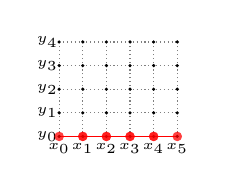
\begin{tikzpicture}[scale=0.3]
                    \foreach \y in {0,...,4} {
                         \draw[gray, densely dotted] (0,\y) -- (5,\y);
                         \node at (-0.5, \y) {\tiny$y_{\y}$};
                         \ifnum \y = 1
                         \draw[red, thin] (0,0) -- (5,0);
                      \fi
                     }
                                         
                     \foreach \x in {0,...,5} {
                         \draw[gray, densely dotted] (\x,0) -- (\x,4);
                         \node at (\x, -0.5) {\tiny$x_{\x}$};
                     }
                     \foreach \x in {0,...,5}
                         \foreach \y in {0,...,4} {
                             \fill (\x,\y) circle (0.0753);
                            \onslide<3->{
                             \ifnum \x=-1 \ifnum \y=0
                                 \fill[red, fill opacity=0.5] (\x,\y) circle (0.2);
                             \fi \fi
                             \ifnum \x=0\ifnum \y=0
                                 \fill[red, fill opacity=0.5] (\x,\y) circle (0.2);
                             \fi \fi
                             \ifnum \x=1 \ifnum \y=0
                                 \fill[red, fill opacity=0.5] (\x,\y) circle (0.2);
                             \fi \fi
                         }
                         \onslide<4->{
                             \ifnum \x=0 \ifnum \y=0
                                 \fill[red, fill opacity=0.5] (\x,\y) circle (0.2);
                             \fi \fi
                             \ifnum \x=1\ifnum \y=0
                                 \fill[red, fill opacity=0.5] (\x,\y) circle (0.2);
                             \fi \fi
                             \ifnum \x=2 \ifnum \y=0
                                 \fill[red, fill opacity=0.5] (\x,\y) circle (0.2);
                             \fi \fi
                         }
                            \onslide<5->{
                                \ifnum \x=1 \ifnum \y=0
                                    \fill[red, fill opacity=0.5] (\x,\y) circle (0.2);
                                \fi \fi
                                \ifnum \x=2\ifnum \y=0
                                    \fill[red, fill opacity=0.5] (\x,\y) circle (0.2);
                                \fi \fi
                                \ifnum \x=3 \ifnum \y=0
                                    \fill[red, fill opacity=0.5] (\x,\y) circle (0.2);
                                \fi \fi
                            }
                            \onslide<6->{
                                \ifnum \x=2 \ifnum \y=0
                                    \fill[red, fill opacity=0.5] (\x,\y) circle (0.2);
                                \fi \fi
                                \ifnum \x=3\ifnum \y=0
                                    \fill[red, fill opacity=0.5] (\x,\y) circle (0.2);
                                \fi \fi
                                \ifnum \x=4 \ifnum \y=0
                                    \fill[red, fill opacity=0.5] (\x,\y) circle (0.2);
                                \fi \fi
                            }
                            \onslide<7->{
                                \ifnum \x=3 \ifnum \y=0
                                    \fill[red, fill opacity=0.5] (\x,\y) circle (0.2);
                                \fi \fi
                                \ifnum \x=4\ifnum \y=0
                                    \fill[red, fill opacity=0.5] (\x,\y) circle (0.2);
                                \fi \fi
                                \ifnum \x=5 \ifnum \y=0
                                    \fill[red, fill opacity=0.5] (\x,\y) circle (0.2);
                                \fi \fi
                            }
                            \onslide<8->{
                                \ifnum \x=4 \ifnum \y=0
                                    \fill[red, fill opacity=0.5] (\x,\y) circle (0.2);
                                \fi \fi
                                \ifnum \x=5\ifnum \y=0
                                    \fill[red, fill opacity=0.5] (\x,\y) circle (0.2);
                                \fi \fi
                                \ifnum \x=6 \ifnum \y=0
                                    \fill[red, fill opacity=0.5] (\x,\y) circle (0.2);
                                \fi \fi
                            }
                         
                         }
                \end{tikzpicture}
            \end{minipage}
            }
        \end{column}
        \hspace{-1.5cm}
       \begin{column}{0.7\textwidth}
            \footnotesize
            
            \vspace{-0.6cm}
            
            \onslide<3->{
                {\tiny
                \begin{align*}
                -\alpha \textcolor{magenta}{u_{-1,0}^{k+\frac{1}{2}}} + (1 + 2\alpha)\textcolor{red}{u_{0,0}^{k+\frac{1}{2}}}
                    - \alpha \textcolor{red}{u_{1,0}^{k+\frac{1}{2}}}
                    = \alpha \textcolor{magenta}{u_{0,-1}^k} + (1 - 2\alpha)\textcolor{blue}{u_{0,0}^k} + \alpha \textcolor{blue}{u_{0,1}^k} + 
                     \frac{\Delta t}{2} S^k
                \end{align*}
                }
            }
            \vspace{-0.611cm}
            \onslide<4->{
                {\tiny
                \begin{align*}
                    -\alpha \textcolor{red}{u_{0,0}^{k+\frac{1}{2}}} + (1 + 2\alpha)\textcolor{red}{u_{1,0}^{k+\frac{1}{2}}}
                    - \alpha \textcolor{red}{u_{2,0}^{k+\frac{1}{2}}}
                    = \alpha \textcolor{magenta}{u_{1,-1}^k} + (1 - 2\alpha)\textcolor{blue}{u_{1,0}^k} + \alpha \textcolor{blue}{u_{1,1}^k} + 
                    \frac{\Delta t}{2} S^k
                \end{align*}
                }
            }
            \vspace{-0.611cm}
            \onslide<5->{
                {\tiny
                \begin{align*}
                    -\alpha \textcolor{red}{u_{1,0}^{k+\frac{1}{2}}} + (1 + 2\alpha)\textcolor{red}{u_{2,0}^{k+\frac{1}{2}}}
                    - \alpha \textcolor{red}{u_{3,0}^{k+\frac{1}{2}}}
                    = \alpha \textcolor{magenta}{u_{2,-1}^k} + (1 - 2\alpha)\textcolor{blue}{u_{2,0}^k} + \alpha \textcolor{blue}{u_{2,1}^k} + 
                    \frac{\Delta t}{2} S^k
                \end{align*}
                }
            }
            \vspace{-0.611cm}
            \onslide<6->{
                {\tiny
                \begin{align*}
                    -\alpha \textcolor{red}{u_{2,0}^{k+\frac{1}{2}}} + (1 + 2\alpha)\textcolor{red}{u_{3,0}^{k+\frac{1}{2}}}
                    - \alpha \textcolor{red}{u_{4,0}^{k+\frac{1}{2}}}
                    = \alpha \textcolor{magenta}{u_{3,-1}^k} + (1 - 2\alpha)\textcolor{blue}{u_{3,0}^k} + \alpha \textcolor{blue}{u_{3,1}^k} +
                    \frac{\Delta t}{2} S^k
                \end{align*}
                }
            }
            \vspace{-0.611cm}
            \onslide<7->{
                {\tiny
                \begin{align*}
                    -\alpha \textcolor{red}{u_{3,0}^{k+\frac{1}{2}}} + (1 + 2\alpha)\textcolor{red}{u_{4,0}^{k+\frac{1}{2}}}
                    - \alpha \textcolor{red}{u_{5,0}^{k+\frac{1}{2}}}
                    = \alpha \textcolor{magenta}{u_{4,-1}^k} + (1 - 2\alpha)\textcolor{blue}{u_{4,0}^k} + \alpha \textcolor{blue}{u_{4,1}^k} +
                    \frac{\Delta t}{2} S^k
                \end{align*}
                }
            }
            \vspace{-0.611cm}
            \onslide<8->{
                {\tiny
                \begin{align*}
                    -\alpha \textcolor{red}{u_{4,0}^{k+\frac{1}{2}}} + (1 + 2\alpha)\textcolor{red}{u_{5,0}^{k+\frac{1}{2}}}
                    - \alpha  \textcolor{magenta}{u_{6,0}^{k+\frac{1}{2}}}
                    = \alpha \textcolor{magenta}{u_{5,-1}^k} + (1 - 2\alpha)\textcolor{blue}{u_{5,0}^k} + \alpha \textcolor{blue}{u_{5,1}^k} +
                    \frac{\Delta t}{2} S^k
                \end{align*}
                }
            }





            
            \onslide<10->{
            Which can be written as a matrix:
            }
            \vspace{-0.3cm}
            \onslide<11->{
                \tiny
                \begin{align*}
                    \begin{bmatrix}
                        -\alpha & 1 + 2\alpha & -\alpha & 0 & 0 & 0 & 0 & 0 \\
                        0 & -\alpha & 1 + 2\alpha & -\alpha & 0 & 0 & 0 & 0 \\
                        0 & 0 & -\alpha & 1 + 2\alpha & -\alpha & 0 & 0 & 0 \\
                        0 & 0 & 0 & -\alpha & 1 + 2\alpha & -\alpha & 0 & 0 \\
                        0 & 0 & 0 & 0 & -\alpha & 1 + 2\alpha & -\alpha & 0 \\
                        0 & 0 & 0 & 0 & 0 & -\alpha & 1 + 2\alpha & -\alpha \\
                    \end{bmatrix}
                    \begin{bmatrix}
                        \textcolor{magenta}{u_{-1,0}^{k+\frac{1}{2}}} \\
                        \textcolor{red}{u_{0,0}^{k+\frac{1}{2}}} \\
                        \textcolor{red}{u_{1,0}^{k+\frac{1}{2}}} \\
                        \textcolor{red}{u_{2,0}^{k+\frac{1}{2}}} \\
                        \textcolor{red}{u_{3,0}^{k+\frac{1}{2}}} \\
                        \textcolor{red}{u_{4,0}^{k+\frac{1}{2}}} \\
                        \textcolor{red}{u_{5,0}^{k+\frac{1}{2}}} \\
                        \textcolor{magenta}{u_{6,0}^{k+\frac{1}{2}}} 
                    \end{bmatrix}
                    =
                    \begin{bmatrix}
                        \textcolor{blue}{b_{0,0}} \\
                        \textcolor{blue}{b_{1,0}} \\
                        \textcolor{blue}{b_{2,0}} \\
                        \textcolor{blue}{b_{3,0}} \\
                        \textcolor{blue}{b_{4,0}} \\
                        \textcolor{blue}{b_{5,0}} \\
                    \end{bmatrix}
                \end{align*}
            }
        \end{column}
    \end{columns}

    \vspace{-1cm}
\end{frame}
\begin{frame}
     \onslide<1->{
                \tiny
                \begin{align*}
                    \begin{bmatrix}
                        -\alpha & 1 + 2\alpha & -\alpha & 0 & 0 & 0 & 0 & 0 \\
                        0 & -\alpha & 1 + 2\alpha & -\alpha & 0 & 0 & 0 & 0 \\
                        0 & 0 & -\alpha & 1 + 2\alpha & -\alpha & 0 & 0 & 0 \\
                        0 & 0 & 0 & -\alpha & 1 + 2\alpha & -\alpha & 0 & 0 \\
                        0 & 0 & 0 & 0 & -\alpha & 1 + 2\alpha & -\alpha & 0 \\
                        0 & 0 & 0 & 0 & 0 & -\alpha & 1 + 2\alpha & -\alpha \\
                    \end{bmatrix}
                    \begin{bmatrix}
                        \textcolor{magenta}{u_{-1,0}^{k+\frac{1}{2}}} \\
                        \textcolor{red}{u_{0,0}^{k+\frac{1}{2}}} \\
                        \textcolor{red}{u_{1,0}^{k+\frac{1}{2}}} \\
                        \textcolor{red}{u_{2,0}^{k+\frac{1}{2}}} \\
                        \textcolor{red}{u_{3,0}^{k+\frac{1}{2}}} \\
                        \textcolor{red}{u_{4,0}^{k+\frac{1}{2}}} \\
                        \textcolor{red}{u_{5,0}^{k+\frac{1}{2}}} \\
                        \textcolor{magenta}{u_{6,0}^{k+\frac{1}{2}}} 
                    \end{bmatrix}
                    =
                    \begin{bmatrix}
                        \textcolor{blue}{b_{0,0}} \\
                        \textcolor{blue}{b_{1,0}} \\
                        \textcolor{blue}{b_{2,0}} \\
                        \textcolor{blue}{b_{3,0}} \\
                        \textcolor{blue}{b_{4,0}} \\
                        \textcolor{blue}{b_{5,0}} \\
                    \end{bmatrix}
                \end{align*}
     }
    \onslide<2->{
        We know the values on the boundaries, so we don't need to include them in the matrix.
             \tiny
                \begin{align*}
                    \begin{bmatrix}
                        1 + \alpha & -\alpha & 0 & 0 & 0 & 0\\
                        -\alpha & 1 + 2\alpha & -\alpha & 0 & 0 & 0\\
                        0 & -\alpha & 1 + 2\alpha & -\alpha & 0 & 0\\
                        0 & 0 & -\alpha & 1 + 2\alpha & -\alpha & 0\\
                        0 & 0 & 0 & -\alpha & 1 + 2\alpha & -\alpha\\
                        0 & 0 & 0 & 0 & -\alpha & 1 + \alpha \\
                    \end{bmatrix}
                    \begin{bmatrix}
                        \textcolor{red}{u_{0,0}^{k+\frac{1}{2}}} \\
                        \textcolor{red}{u_{1,0}^{k+\frac{1}{2}}} \\
                        \textcolor{red}{u_{2,0}^{k+\frac{1}{2}}} \\
                        \textcolor{red}{u_{3,0}^{k+\frac{1}{2}}} \\
                        \textcolor{red}{u_{4,0}^{k+\frac{1}{2}}} \\
                        \textcolor{red}{u_{5,0}^{k+\frac{1}{2}}} \\
                    \end{bmatrix}
                    =
                    \begin{bmatrix}
                        \textcolor{blue}{b_{0,0}} \\
                        \textcolor{blue}{b_{1,0}} \\
                        \textcolor{blue}{b_{2,0}} \\
                        \textcolor{blue}{b_{3,0}} \\
                        \textcolor{blue}{b_{4,0}} \\
                        \textcolor{blue}{b_{5,0}} \\
                    \end{bmatrix}
                \end{align*}
    }
            
\end{frame}

\begin{frame}
    \vspace{-0.8cm}   
    Let's fix $j = 1$ and write the equations for $0 \leq i \leq 5$.
    
    \begin{columns}
        \begin{column}{0.3\textwidth}
            % Place both figures in a row here
            \begin{minipage}{0.2\textwidth}
                $k$
                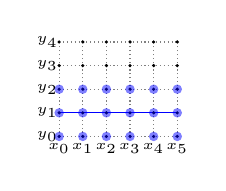
\begin{tikzpicture}[scale=0.3]
                    \foreach \y in {0,...,4} {
                         \draw[gray, densely dotted] (0,\y) -- (5,\y);
                         \node at (-0.5, \y) {\tiny$y_{\y}$};
                         \ifnum \y = 1
                            \draw[blue, thin] (0,1) -- (5,1);
                         \fi
                     }
                                         
                     \foreach \x in {0,...,5} {
                         \draw[gray, densely dotted] (\x,0) -- (\x,4);
                         \node at (\x, -0.5) {\tiny$x_{\x}$};
                     }
                     \foreach \x in {0,...,5}
                         \foreach \y in {0,...,4} {
                             \fill (\x,\y) circle (0.0753);
                             \onslide<3->{  
                             \ifnum \x=0 \ifnum \y=0
                                 \fill[blue, fill opacity=0.5] (\x,\y) circle (0.2);
                             \fi \fi
                             \ifnum \x=0\ifnum \y=1
                                 \fill[blue, fill opacity=0.5] (\x,\y) circle (0.2);
                             \fi \fi
                             \ifnum \x=0 \ifnum \y=2
                                 \fill[blue, fill opacity=0.5] (\x,\y) circle (0.2);
                             \fi \fi
                             }
                            \onslide<4->{
                                \ifnum \x=1 \ifnum \y=0
                                    \fill[blue, fill opacity=0.5] (\x,\y) circle (0.2);
                                \fi \fi
                                \ifnum \x=1\ifnum \y=1
                                    \fill[blue, fill opacity=0.5] (\x,\y) circle (0.2);
                                \fi \fi
                                \ifnum \x=1 \ifnum \y=2
                                    \fill[blue, fill opacity=0.5] (\x,\y) circle (0.2);
                                \fi \fi
                                }
                            \onslide<5->{
                                \ifnum \x=2 \ifnum \y=0
                                    \fill[blue, fill opacity=0.5] (\x,\y) circle (0.2);
                                \fi \fi
                                \ifnum \x=2\ifnum \y=1
                                    \fill[blue, fill opacity=0.5] (\x,\y) circle (0.2);
                                \fi \fi
                                \ifnum \x=2 \ifnum \y=2
                                    \fill[blue, fill opacity=0.5] (\x,\y) circle (0.2);
                                \fi \fi
                                }
                            \onslide<6->{
                                \ifnum \x=3 \ifnum \y=0
                                    \fill[blue, fill opacity=0.5] (\x,\y) circle (0.2);
                                \fi \fi
                                \ifnum \x=3\ifnum \y=1
                                    \fill[blue, fill opacity=0.5] (\x,\y) circle (0.2);
                                \fi \fi
                                \ifnum \x=3 \ifnum \y=2
                                    \fill[blue, fill opacity=0.5] (\x,\y) circle (0.2);
                                \fi \fi
                                }
                            \onslide<7->{
                                \ifnum \x=4 \ifnum \y=0
                                    \fill[blue, fill opacity=0.5] (\x,\y) circle (0.2);
                                \fi \fi
                                \ifnum \x=4\ifnum \y=1
                                    \fill[blue, fill opacity=0.5] (\x,\y) circle (0.2);
                                \fi \fi
                                \ifnum \x=4 \ifnum \y=2
                                    \fill[blue, fill opacity=0.5] (\x,\y) circle (0.2);
                                \fi \fi
                            }
                            \onslide<8->{
                                \ifnum \x=5 \ifnum \y=0
                                    \fill[blue, fill opacity=0.5] (\x,\y) circle (0.2);
                                \fi \fi
                                \ifnum \x=5\ifnum \y=1
                                    \fill[blue, fill opacity=0.5] (\x,\y) circle (0.2);
                                \fi \fi
                                \ifnum \x=5 \ifnum \y=2
                                    \fill[blue, fill opacity=0.5] (\x,\y) circle (0.2);
                                \fi \fi
                            }


                         }
                         
                 \end{tikzpicture}
                \end{minipage}\\
            \vspace{-0.2cm}
            \onslide<2->{
            \begin{center}
               
            \end{center}
            \vspace{1.1cm}
            \begin{minipage}{0.3\textwidth}
                $k+\frac{1}{2}$
                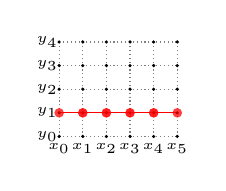
\begin{tikzpicture}[scale=0.3]
                    \foreach \y in {0,...,4} {
                         \draw[gray, densely dotted] (0,\y) -- (5,\y);
                         \node at (-0.5, \y) {\tiny$y_{\y}$};
                         \ifnum \y = 1
                         \draw[red, thin] (0,1) -- (5,1);
                      \fi
                     }
                                         
                     \foreach \x in {0,...,5} {
                         \draw[gray, densely dotted] (\x,0) -- (\x,4);
                         \node at (\x, -0.5) {\tiny$x_{\x}$};
                     }
                     \foreach \x in {0,...,5}
                         \foreach \y in {0,...,4} {
                             \fill (\x,\y) circle (0.0753);
                            \onslide<3->{
                             \ifnum \x=-1 \ifnum \y=1
                                 \fill[red, fill opacity=0.5] (\x,\y) circle (0.2);
                             \fi \fi
                             \ifnum \x=0\ifnum \y=1
                                 \fill[red, fill opacity=0.5] (\x,\y) circle (0.2);
                             \fi \fi
                             \ifnum \x=1 \ifnum \y=1
                                 \fill[red, fill opacity=0.5] (\x,\y) circle (0.2);
                             \fi \fi
                         }
                         \onslide<4->{
                             \ifnum \x=0 \ifnum \y=1
                                 \fill[red, fill opacity=0.5] (\x,\y) circle (0.2);
                             \fi \fi
                             \ifnum \x=1\ifnum \y=1
                                 \fill[red, fill opacity=0.5] (\x,\y) circle (0.2);
                             \fi \fi
                             \ifnum \x=2 \ifnum \y=1
                                 \fill[red, fill opacity=0.5] (\x,\y) circle (0.2);
                             \fi \fi
                         }
                            \onslide<5->{
                                \ifnum \x=1 \ifnum \y=1
                                    \fill[red, fill opacity=0.5] (\x,\y) circle (0.2);
                                \fi \fi
                                \ifnum \x=2\ifnum \y=1
                                    \fill[red, fill opacity=0.5] (\x,\y) circle (0.2);
                                \fi \fi
                                \ifnum \x=3 \ifnum \y=1
                                    \fill[red, fill opacity=0.5] (\x,\y) circle (0.2);
                                \fi \fi
                            }
                            \onslide<6->{
                                \ifnum \x=2 \ifnum \y=1
                                    \fill[red, fill opacity=0.5] (\x,\y) circle (0.2);
                                \fi \fi
                                \ifnum \x=3\ifnum \y=1
                                    \fill[red, fill opacity=0.5] (\x,\y) circle (0.2);
                                \fi \fi
                                \ifnum \x=4 \ifnum \y=1
                                    \fill[red, fill opacity=0.5] (\x,\y) circle (0.2);
                                \fi \fi
                            }
                            \onslide<7->{
                                \ifnum \x=3 \ifnum \y=1
                                    \fill[red, fill opacity=0.5] (\x,\y) circle (0.2);
                                \fi \fi
                                \ifnum \x=4\ifnum \y=1
                                    \fill[red, fill opacity=0.5] (\x,\y) circle (0.2);
                                \fi \fi
                                \ifnum \x=5 \ifnum \y=1
                                    \fill[red, fill opacity=0.5] (\x,\y) circle (0.2);
                                \fi \fi
                            }
                            \onslide<8->{
                                \ifnum \x=4 \ifnum \y=1
                                    \fill[red, fill opacity=0.5] (\x,\y) circle (0.2);
                                \fi \fi
                                \ifnum \x=5\ifnum \y=1
                                    \fill[red, fill opacity=0.5] (\x,\y) circle (0.2);
                                \fi \fi
                                \ifnum \x=6 \ifnum \y=1
                                    \fill[red, fill opacity=0.5] (\x,\y) circle (0.2);
                                \fi \fi
                            }
                         
                         }
                \end{tikzpicture}
            \end{minipage}
            }
        \end{column}
        \hspace{-1.5cm}
       \begin{column}{0.7\textwidth}
            \footnotesize
            
            \vspace{-0.6cm}
            
            \onslide<3->{
                {\tiny
                \begin{align*}
                -\alpha \textcolor{magenta}{u_{-1,1}^{k+\frac{1}{2}}} + (1 + 2\alpha)\textcolor{red}{u_{0,1}^{k+\frac{1}{2}}}
                    - \alpha \textcolor{red}{u_{1,1}^{k+\frac{1}{2}}}
                    = \alpha \textcolor{blue}{u_{0,0}^k} + (1 - 2\alpha)\textcolor{blue}{u_{0,1}^k} + \alpha \textcolor{blue}{u_{0,2}^k} + 
                     \frac{\Delta t}{2} S^k
                \end{align*}
                }
            }
            \vspace{-0.611cm}
            \onslide<4->{
                {\tiny
                \begin{align*}
                    -\alpha \textcolor{red}{u_{0,1}^{k+\frac{1}{2}}} + (1 + 2\alpha)\textcolor{red}{u_{1,1}^{k+\frac{1}{2}}}
                    - \alpha \textcolor{red}{u_{2,1}^{k+\frac{1}{2}}}
                    = \alpha \textcolor{blue}{u_{1,0}^k} + (1 - 2\alpha)\textcolor{blue}{u_{1,1}^k} + \alpha \textcolor{blue}{u_{1,2}^k} + 
                    \frac{\Delta t}{2} S^k
                \end{align*}
                }
            }
            \vspace{-0.611cm}
            \onslide<5->{
                {\tiny
                \begin{align*}
                    -\alpha \textcolor{red}{u_{1,1}^{k+\frac{1}{2}}} + (1 + 2\alpha)\textcolor{red}{u_{2,1}^{k+\frac{1}{2}}}
                    - \alpha \textcolor{red}{u_{3,1}^{k+\frac{1}{2}}}
                    = \alpha \textcolor{blue}{u_{2,0}^k} + (1 - 2\alpha)\textcolor{blue}{u_{2,1}^k} + \alpha \textcolor{blue}{u_{2,2}^k} + 
                    \frac{\Delta t}{2} S^k
                \end{align*}
                }
            }
            \vspace{-0.611cm}
            \onslide<6->{
                {\tiny
                \begin{align*}
                    -\alpha \textcolor{red}{u_{2,1}^{k+\frac{1}{2}}} + (1 + 2\alpha)\textcolor{red}{u_{3,1}^{k+\frac{1}{2}}}
                    - \alpha \textcolor{red}{u_{4,1}^{k+\frac{1}{2}}}
                    = \alpha \textcolor{blue}{u_{3,0}^k} + (1 - 2\alpha)\textcolor{blue}{u_{3,1}^k} + \alpha \textcolor{blue}{u_{3,2}^k} +
                    \frac{\Delta t}{2} S^k
                \end{align*}
                }
            }
            \vspace{-0.611cm}
            \onslide<7->{
                {\tiny
                \begin{align*}
                    -\alpha \textcolor{red}{u_{3,1}^{k+\frac{1}{2}}} + (1 + 2\alpha)\textcolor{red}{u_{4,1}^{k+\frac{1}{2}}}
                    - \alpha \textcolor{red}{u_{5,1}^{k+\frac{1}{2}}}
                    = \alpha \textcolor{blue}{u_{4,0}^k} + (1 - 2\alpha)\textcolor{blue}{u_{4,1}^k} + \alpha \textcolor{blue}{u_{4,2}^k} +
                    \frac{\Delta t}{2} S^k
                \end{align*}
                }
            }
            \vspace{-0.611cm}
            \onslide<8->{
                {\tiny
                \begin{align*}
                    -\alpha \textcolor{red}{u_{4,1}^{k+\frac{1}{2}}} + (1 + 2\alpha)\textcolor{red}{u_{5,1}^{k+\frac{1}{2}}}
                    - \alpha  \textcolor{magenta}{u_{6,1}^{k+\frac{1}{2}}}
                    = \alpha \textcolor{blue}{u_{5,0}^k} + (1 - 2\alpha)\textcolor{blue}{u_{5,1}^k} + \alpha \textcolor{blue}{u_{5,2}^k} +
                    \frac{\Delta t}{2} S^k
                \end{align*}
                }
            }





            
            \onslide<10->{
            Which can be written as a matrix:
            }
            \vspace{-0.3cm}
            \onslide<11->{
                \tiny
                \begin{align*}
                    \begin{bmatrix}
                        -\alpha & 1 + 2\alpha & -\alpha & 0 & 0 & 0 & 0 & 0 \\
                        0 & -\alpha & 1 + 2\alpha & -\alpha & 0 & 0 & 0 & 0 \\
                        0 & 0 & -\alpha & 1 + 2\alpha & -\alpha & 0 & 0 & 0 \\
                        0 & 0 & 0 & -\alpha & 1 + 2\alpha & -\alpha & 0 & 0 \\
                        0 & 0 & 0 & 0 & -\alpha & 1 + 2\alpha & -\alpha & 0 \\
                        0 & 0 & 0 & 0 & 0 & -\alpha & 1 + 2\alpha & -\alpha \\
                    \end{bmatrix}
                    \begin{bmatrix}
                        \textcolor{magenta}{u_{-1,1}^{k+\frac{1}{2}}} \\
                        \textcolor{red}{u_{0,1}^{k+\frac{1}{2}}} \\
                        \textcolor{red}{u_{1,1}^{k+\frac{1}{2}}} \\
                        \textcolor{red}{u_{2,1}^{k+\frac{1}{2}}} \\
                        \textcolor{red}{u_{3,1}^{k+\frac{1}{2}}} \\
                        \textcolor{red}{u_{4,1}^{k+\frac{1}{2}}} \\
                        \textcolor{red}{u_{5,1}^{k+\frac{1}{2}}} \\
                        \textcolor{magenta}{u_{6,1}^{k+\frac{1}{2}}} 
                    \end{bmatrix}
                    =
                    \begin{bmatrix}
                        \textcolor{blue}{b_{0,1}} \\
                        \textcolor{blue}{b_{1,1}} \\
                        \textcolor{blue}{b_{2,1}} \\
                        \textcolor{blue}{b_{3,1}} \\
                        \textcolor{blue}{b_{4,1}} \\
                        \textcolor{blue}{b_{5,1}} \\
                    \end{bmatrix}
                \end{align*}
            }
        \end{column}
    \end{columns}

    \vspace{-1cm}
\end{frame}

\begin{frame}
     \onslide<1->{
                   \tiny
                \begin{align*}
                    \begin{bmatrix}
                        -\alpha & 1 + 2\alpha & -\alpha & 0 & 0 & 0 & 0 & 0 \\
                        0 & -\alpha & 1 + 2\alpha & -\alpha & 0 & 0 & 0 & 0 \\
                        0 & 0 & -\alpha & 1 + 2\alpha & -\alpha & 0 & 0 & 0 \\
                        0 & 0 & 0 & -\alpha & 1 + 2\alpha & -\alpha & 0 & 0 \\
                        0 & 0 & 0 & 0 & -\alpha & 1 + 2\alpha & -\alpha & 0 \\
                        0 & 0 & 0 & 0 & 0 & -\alpha & 1 + 2\alpha & -\alpha \\
                    \end{bmatrix}
                    \begin{bmatrix}
                        \textcolor{magenta}{u_{-1,1}^{k+\frac{1}{2}}} \\
                        \textcolor{red}{u_{0,1}^{k+\frac{1}{2}}} \\
                        \textcolor{red}{u_{1,1}^{k+\frac{1}{2}}} \\
                        \textcolor{red}{u_{2,1}^{k+\frac{1}{2}}} \\
                        \textcolor{red}{u_{3,1}^{k+\frac{1}{2}}} \\
                        \textcolor{red}{u_{4,1}^{k+\frac{1}{2}}} \\
                        \textcolor{red}{u_{5,1}^{k+\frac{1}{2}}} \\
                        \textcolor{magenta}{u_{6,1}^{k+\frac{1}{2}}} 
                    \end{bmatrix}
                    =
                    \begin{bmatrix}
                        \textcolor{blue}{b_{0,1}} \\
                        \textcolor{blue}{b_{1,1}} \\
                        \textcolor{blue}{b_{2,1}} \\
                        \textcolor{blue}{b_{3,1}} \\
                        \textcolor{blue}{b_{4,1}} \\
                        \textcolor{blue}{b_{5,1}} \\
                    \end{bmatrix}
                \end{align*}
     }
    \onslide<2->{
        We know the values on the boundaries, so we don't need to include them in the matrix.
             \tiny
                \begin{align*}
                    \begin{bmatrix}
                        1 + \alpha & -\alpha & 0 & 0 & 0 & 0\\
                        -\alpha & 1 + 2\alpha & -\alpha & 0 & 0 & 0\\
                        0 & -\alpha & 1 + 2\alpha & -\alpha & 0 & 0\\
                        0 & 0 & -\alpha & 1 + 2\alpha & -\alpha & 0\\
                        0 & 0 & 0 & -\alpha & 1 + 2\alpha & -\alpha\\
                        0 & 0 & 0 & 0 & -\alpha & 1 + \alpha \\
                    \end{bmatrix}
                    \begin{bmatrix}
                        \textcolor{red}{u_{0,1}^{k+\frac{1}{2}}} \\
                        \textcolor{red}{u_{1,1}^{k+\frac{1}{2}}} \\
                        \textcolor{red}{u_{2,1}^{k+\frac{1}{2}}} \\
                        \textcolor{red}{u_{3,1}^{k+\frac{1}{2}}} \\
                        \textcolor{red}{u_{4,1}^{k+\frac{1}{2}}} \\
                        \textcolor{red}{u_{5,1}^{k+\frac{1}{2}}} \\
                    \end{bmatrix}
                    =
                    \begin{bmatrix}
                        \textcolor{blue}{b_{0,1}} \\
                        \textcolor{blue}{b_{1,1}} \\
                        \textcolor{blue}{b_{2,1}} \\
                        \textcolor{blue}{b_{3,1}} \\
                        \textcolor{blue}{b_{4,1}} \\
                        \textcolor{blue}{b_{5,1}} \\
                    \end{bmatrix}
                \end{align*}
    }
            
\end{frame}

\begin{frame}
    \vspace{-0.8cm}   
    We get one system of equations for each $j$ value.
    
    \begin{columns}
        \begin{column}{0.3\textwidth}
            % Place both figures in a row here
            \begin{minipage}{0.48\textwidth}
                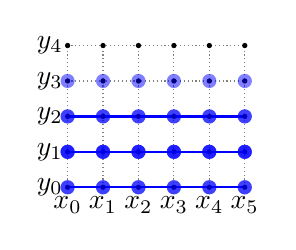
\begin{tikzpicture}[scale=0.45]
                    \foreach \y in {0,...,4} {
                         \draw[gray, densely dotted] (0,\y) -- (5,\y);
                         \node at (-0.5, \y) {$y_{\y}$};
                         \onslide<2->{
                         \ifnum \y = 0 
                         \draw[blue, thick] (0,\y) -- (5,\y);
                          \fi
                         }
                         \onslide<3->{
                            \ifnum \y = 1
                            \draw[blue, thick] (0,\y) -- (5,\y);
                            \fi
                         }
                         \onslide<4->{
                            \ifnum \y = 2
                            \draw[blue, thick] (0,\y) -- (5,\y);
                            \fi
                         }
                     } 
                                         
                     \foreach \x in {0,...,5} {
                         \draw[gray, densely dotted] (\x,0) -- (\x,4);
                         \node at (\x, -0.5) {$x_{\x}$};
                     }
                     \foreach \x in {0,...,5}
                         \foreach \y in {0,...,4} {
                             \fill (\x,\y) circle (0.0753); 
                             \onslide<2->{
                             \ifnum  \y=-1 \ifnum  \x>-1 \ifnum  \x<6
                                 \fill[blue, fill opacity=0.5] (\x,\y) circle (0.2);
                            \fi \fi \fi
                            \ifnum  \y=0  \ifnum  \x>-1 \ifnum  \x<6
                                \fill[blue, fill opacity=0.5] (\x,\y) circle (0.2);
                                \fi \fi \fi
                            \ifnum  \y=1 \ifnum  \x>-1 \ifnum  \x<6
                                \fill[blue, fill opacity=0.5] (\x,\y) circle (0.2);
                                \fi \fi \fi 
                             }
                             \onslide<3->{
                                \ifnum  \y=0 \ifnum  \x>-1 \ifnum  \x<6
                                    \fill[blue, fill opacity=0.5] (\x,\y) circle (0.2);
                                \fi \fi \fi
                                \ifnum  \y=1  \ifnum  \x>-1 \ifnum  \x<6
                                    \fill[blue, fill opacity=0.5] (\x,\y) circle (0.2);
                                    \fi \fi \fi
                                \ifnum  \y=2 \ifnum  \x>-1 \ifnum  \x<6
                                    \fill[blue, fill opacity=0.5] (\x,\y) circle (0.2);
                                    \fi \fi \fi 
                                 }
                           \onslide<4->{
                                \ifnum  \y=1 \ifnum  \x>-1 \ifnum  \x<6
                                    \fill[blue, fill opacity=0.5] (\x,\y) circle (0.2);
                                \fi \fi \fi
                                \ifnum  \y=2  \ifnum  \x>-1 \ifnum  \x<6
                                    \fill[blue, fill opacity=0.5] (\x,\y) circle (0.2);
                                    \fi \fi \fi
                                \ifnum  \y=3 \ifnum  \x>-1 \ifnum  \x<6
                                    \fill[blue, fill opacity=0.5] (\x,\y) circle (0.2);
                                    \fi \fi \fi 
                                 


                           }
                         }
                         
                 \end{tikzpicture}
                \end{minipage}\\
            \vspace{-0.2cm}
           
            \begin{center}
                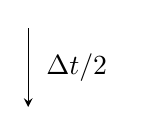
\begin{tikzpicture}[>=stealth]
                    \draw[->] (0,0) -- (0,-1) node[midway, right, xshift=3pt] {$\Delta t/2$};
                \end{tikzpicture}
            \end{center}
            \vspace{-0.2cm}
            \begin{minipage}{0.48\textwidth}
                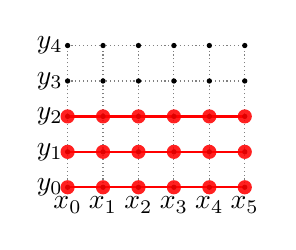
\begin{tikzpicture}[scale=0.45]
                    \foreach \y in {0,...,4} {
                         \draw[gray, densely dotted] (0,\y) -- (5,\y);
                         \node at (-0.5, \y) {$y_{\y}$};
                         \onslide<2->{
                         \ifnum \y = 0
                         \draw[red, thick] (0,\y) -- (5,\y);
                      \fi}
                        \onslide<3->{
                            \ifnum \y = 1
                            \draw[red, thick] (0,\y) -- (5,\y);
                            \fi
                        }
                        \onslide<4->{
                            \ifnum \y = 2
                            \draw[red, thick] (0,\y) -- (5,\y);
                            \fi
                        }
                     }
                                         
                     \foreach \x in {0,...,5} {
                         \draw[gray, densely dotted] (\x,0) -- (\x,4);
                         \node at (\x, -0.5) {$x_{\x}$};

                     }
                     \foreach \x in {0,...,5}
                         \foreach \y in {0,...,4} {
                             \fill (\x,\y) circle (0.0753); 
                             \onslide<2->{
                             \ifnum \y=0
                            \fill[red, fill opacity=0.875] (\x,\y) circle (0.2);
                            \fi
                            }
                            \onslide<3->{
                                \ifnum \y=1
                                \fill[red, fill opacity=0.875] (\x,\y) circle (0.2);
                                \fi
                            }
                            \onslide<4->{
                                \ifnum \y=2
                                \fill[red, fill opacity=0.875] (\x,\y) circle (0.2);
                                \fi
                            }
                         }
                \end{tikzpicture}
            \end{minipage}
            
        \end{column}
        \hspace{-0.8cm}
       \begin{column}{0.7\textwidth}
            %\footnotesize
            %we need smaller font size. let's try even smaller. Let's try tiny.
            \tiny
          \vspace{-1.5cm}  
          \onslide<2->{
                    \tiny
                \begin{align*}
                    \begin{bmatrix}
                        1 + \alpha & -\alpha & 0 & 0 & 0 & 0\\
                        -\alpha & 1 + 2\alpha & -\alpha & 0 & 0 & 0\\
                        0 & -\alpha & 1 + 2\alpha & -\alpha & 0 & 0\\
                        0 & 0 & -\alpha & 1 + 2\alpha & -\alpha & 0\\
                        0 & 0 & 0 & -\alpha & 1 + 2\alpha & -\alpha\\
                        0 & 0 & 0 & 0 & -\alpha & 1 + \alpha \\
                    \end{bmatrix}
                    \begin{bmatrix}
                        \textcolor{red}{u_{0,0}^{k+\frac{1}{2}}} \\
                        \textcolor{red}{u_{1,0}^{k+\frac{1}{2}}} \\
                        \textcolor{red}{u_{2,0}^{k+\frac{1}{2}}} \\
                        \textcolor{red}{u_{3,0}^{k+\frac{1}{2}}} \\
                        \textcolor{red}{u_{4,0}^{k+\frac{1}{2}}} \\
                        \textcolor{red}{u_{5,0}^{k+\frac{1}{2}}} \\
                    \end{bmatrix}
                    =
                    \begin{bmatrix}
                        \textcolor{blue}{b_{0,0}} \\
                        \textcolor{blue}{b_{1,0}} \\
                        \textcolor{blue}{b_{2,0}} \\
                        \textcolor{blue}{b_{3,0}} \\
                        \textcolor{blue}{b_{4,0}} \\
                        \textcolor{blue}{b_{5,0}} \\
                    \end{bmatrix}
                \end{align*}
          }
                \vspace{-0.5cm}
                \onslide<3->{
              \tiny
                \begin{align*}
                    \begin{bmatrix}
                        1 + \alpha & -\alpha & 0 & 0 & 0 & 0\\
                        -\alpha & 1 + 2\alpha & -\alpha & 0 & 0 & 0\\
                        0 & -\alpha & 1 + 2\alpha & -\alpha & 0 & 0\\
                        0 & 0 & -\alpha & 1 + 2\alpha & -\alpha & 0\\
                        0 & 0 & 0 & -\alpha & 1 + 2\alpha & -\alpha\\
                        0 & 0 & 0 & 0 & -\alpha & 1 + \alpha \\
                    \end{bmatrix}
                    \begin{bmatrix}
                        \textcolor{red}{u_{0,1}^{k+\frac{1}{2}}} \\
                        \textcolor{red}{u_{1,1}^{k+\frac{1}{2}}} \\
                        \textcolor{red}{u_{2,1}^{k+\frac{1}{2}}} \\
                        \textcolor{red}{u_{3,1}^{k+\frac{1}{2}}} \\
                        \textcolor{red}{u_{4,1}^{k+\frac{1}{2}}} \\
                        \textcolor{red}{u_{5,1}^{k+\frac{1}{2}}} \\
                    \end{bmatrix}
                    =
                    \begin{bmatrix}
                        \textcolor{blue}{b_{0,1}} \\
                        \textcolor{blue}{b_{1,1}} \\
                        \textcolor{blue}{b_{2,1}} \\
                        \textcolor{blue}{b_{3,1}} \\
                        \textcolor{blue}{b_{4,1}} \\
                        \textcolor{blue}{b_{5,1}} \\
                    \end{bmatrix}
                \end{align*}
                }
                \vspace{-0.5cm}
                \onslide<4->{
               \tiny
                \begin{align*}
                    \begin{bmatrix}
                        1 + \alpha & -\alpha & 0 & 0 & 0 & 0\\
                        -\alpha & 1 + 2\alpha & -\alpha & 0 & 0 & 0\\
                        0 & -\alpha & 1 + 2\alpha & -\alpha & 0 & 0\\
                        0 & 0 & -\alpha & 1 + 2\alpha & -\alpha & 0\\
                        0 & 0 & 0 & -\alpha & 1 + 2\alpha & -\alpha\\
                        0 & 0 & 0 & 0 & -\alpha & 1 + \alpha \\
                    \end{bmatrix}
                    \begin{bmatrix}
                        \textcolor{red}{u_{0,2}^{k+\frac{1}{2}}} \\
                        \textcolor{red}{u_{1,2}^{k+\frac{1}{2}}} \\
                        \textcolor{red}{u_{2,2}^{k+\frac{1}{2}}} \\
                        \textcolor{red}{u_{3,2}^{k+\frac{1}{2}}} \\
                        \textcolor{red}{u_{4,2}^{k+\frac{1}{2}}} \\
                        \textcolor{red}{u_{5,2}^{k+\frac{1}{2}}} \\
                    \end{bmatrix}
                    =
                    \begin{bmatrix}
                        \textcolor{blue}{b_{0,2}} \\
                        \textcolor{blue}{b_{1,2}} \\
                        \textcolor{blue}{b_{2,2}} \\
                        \textcolor{blue}{b_{3,2}} \\
                        \textcolor{blue}{b_{4,2}} \\
                        \textcolor{blue}{b_{5,2}} \\
                    \end{bmatrix}
                \end{align*}
                }
                \vspace{-3.5cm}
        \end{column}
    \end{columns}
    
    \vspace{0.1cm}
    \small
   
\end{frame}

\begin{frame}
Each tridiagonal system can be solved using Thomas algorithm.

\end{frame}

\end{document}
